%%%%%%%%%%%%%%%%%%%%%%%%%%%%%%%%%%%%% 
%% LE2I beamer template
%% Guillaume Lemaitre, October 2014
%%%%%%%%%%%%%%%%%%%%%%%%%%%%%%%%%%%%% 

\documentclass{beamer}

\usepackage[utf8]{inputenc}
\usepackage[T1]{fontenc} 
\usetheme{le2i} 

%% The amssymb package provides various useful mathematical symbols
\usepackage{amssymb}
%% The amsthm package provides extended theorem environments
\usepackage{amsthm}

%% amsmath for math environment
\usepackage{amsmath}

\DeclareMathOperator*{\argmin}{arg\,min}
\DeclareMathOperator*{\argmax}{arg\,max}
\DeclareMathOperator*{\sign}{sign}

%% figure package
\usepackage{epsf,graphicx}
\usepackage{epstopdf}
\usepackage{subfigure}
\usepackage{transparent}

%% In order to draw some graphs
\usepackage{tikz,xifthen}
\usepackage{tikz-qtree}
\usepackage{adjustbox}
\usetikzlibrary{decorations.pathmorphing}
\usetikzlibrary{fit}
\usetikzlibrary{backgrounds}
\usetikzlibrary{shapes,arrows,shadows}
\usetikzlibrary{calc,decorations.pathreplacing,decorations.markings,positioning}
\usetikzlibrary{snakes,decorations.text,shapes,patterns}
% \usepackage{scalefnt,lmodern,booktabs}

%% Package for cross and tick symbols
\usepackage{pifont}
\newcommand{\tick}{\color{green!60!black!80}\ding{51}}
\newcommand{\cross}{\color{red!60!black!80}\ding{55}}

\title{Color Image Processing}
\author{Guillaume Lemaitre}
%\date{Define the event \\ day\textsuperscript{th} Month Year}

\institute{Universit\'e de Bourgogne} 

%% Uncomment if you want to avoid thousand of bullet inside the menu
% \usepackage{etoolbox}
% \makeatletter
% \patchcmd{\slideentry}{\advance\beamer@xpos by1\relax}{}{}{}
% \def\beamer@subsectionentry#1#2#3#4#5{\advance\beamer@xpos by1\relax}%
% \makeatother

\begin{document}

% Show the title page
\begin{frame}
  \titlepage
\end{frame}

% Show the table of contents
\begin{frame}
  \tableofcontents[sectionstyle=show,subsectionstyle=show,subsubsectionstyle=hide]
\end{frame}

%---------------------
\section{Color fundamentals}
\begin{frame}
\frametitle{Color Image Processing}
\begin{block}{Why color? }
\begin{itemize}
	\item Color is a powerful descriptor for object identification and extraction
	\item Human capability for perceiving of thousands of color shades and intensities
\end{itemize}
\end{block}
\begin{block}{Color fundamentals}
\begin{itemize}
	\item Splitting of white light, while passes through glass prism
	\item[]
	\centering{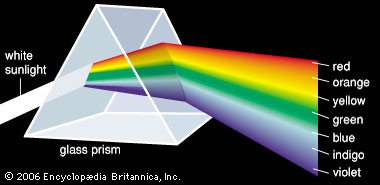
\includegraphics[width = 0.6\textwidth , height = 0.2\textheight]{images/L6_color_prism.jpg}}	
	\item[] Visible range
\end{itemize}
\end{block}
\end{frame}
%------------
\begin{frame}
\frametitle{Color fundamentals}
\begin{block}{Visible light}
\begin{itemize}
	\item[]
	\centering{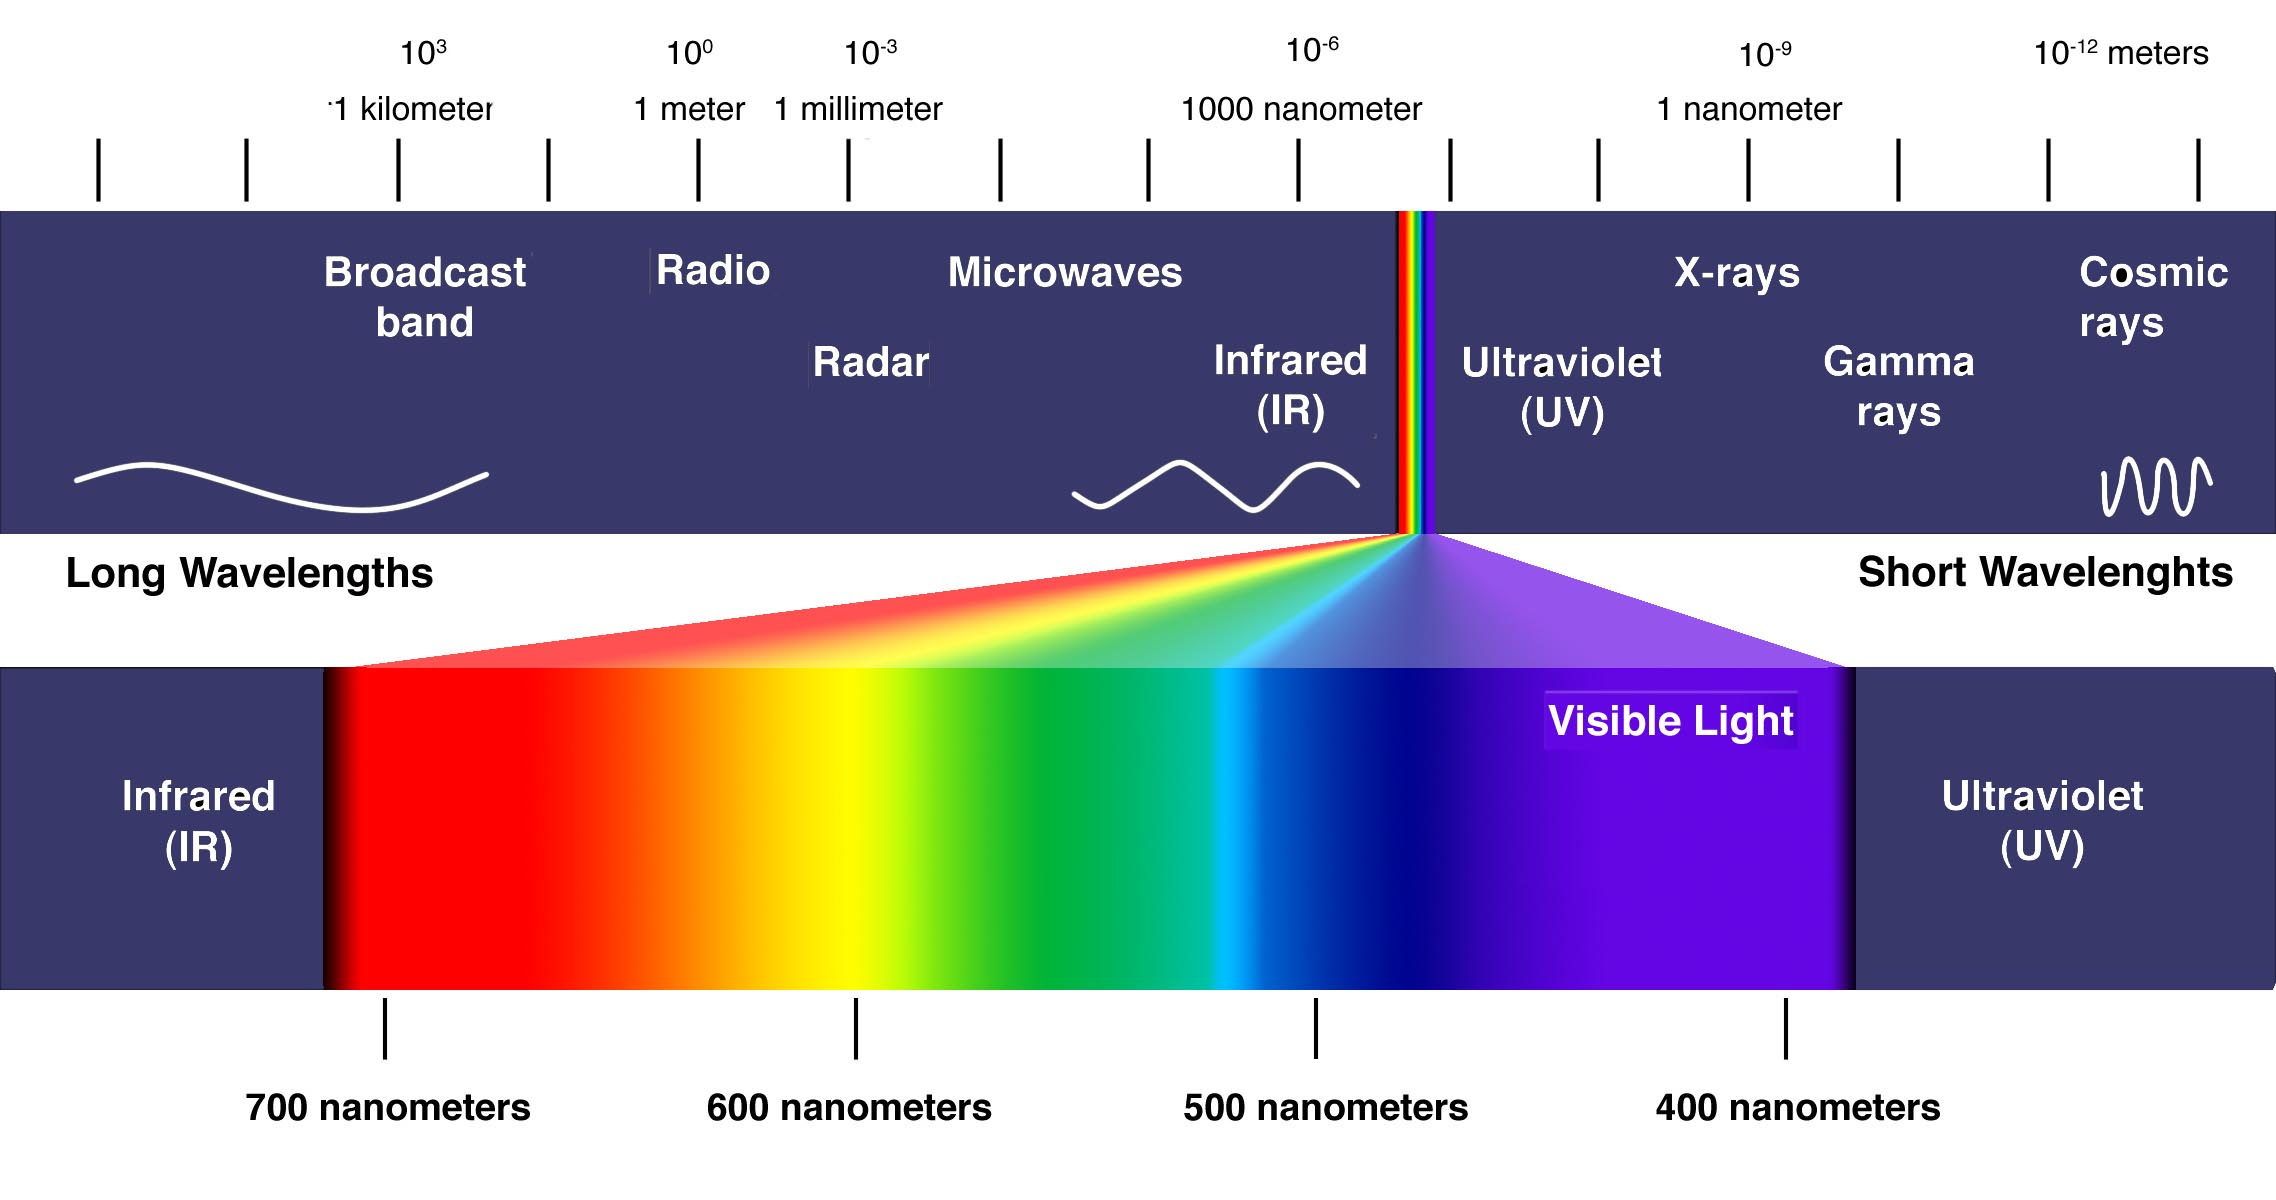
\includegraphics[scale=0.45]{images/L6_electromagnetic.jpg}}
\end{itemize}
\end{block}
\end{frame}
%------------
\begin{frame}
\frametitle{Color fundamentals}
\begin{block}{Color perception}
\begin{itemize}
		\item The perceive colors from an object are determined by the nature of light reflected from the object
		\begin{itemize}
		\item If an object reflects light that balanced from all visible wavelengths, object is perceived as white
		\item If an object reflects light mainly in the range of 575 to 625 nm, the object is perceived as red  
		\end{itemize}
\end{itemize}

\end{block}
\end{frame}

%------------
\begin{frame}
\frametitle{Color fundamentals}
\begin{block}{Chromatic light}
\begin{itemize}
	\item Achromatic light(free of color), its only attribute is its intensity
	\item Chromatic light spans the electromagnetic spectrum from approximately 400 to 700 nm
	\item The quality of chromatic light is described by radiance, luminance, and brightness
	\begin{itemize}
		\item Radiance is the total amount of energy that flows from the light source, measured in $W$
		\item Luminance is the measure of the energy that observer receives from the light, $lm$ (lumens)
		\item Brightness is a subjective descriptor that is impossible to measure
	\end{itemize}
\end{itemize}
\end{block}
\end{frame}
%-------------
\begin{frame}
\frametitle{Color fundamentals}
\begin{block}{Primary colors}
\begin{itemize}
	\item Why so called primary colors, Red (R), Green (G), and Blue (B) ? 
	\begin{itemize}
	\item Average absorption of light by human eyes cones
	\item[] \centering{
	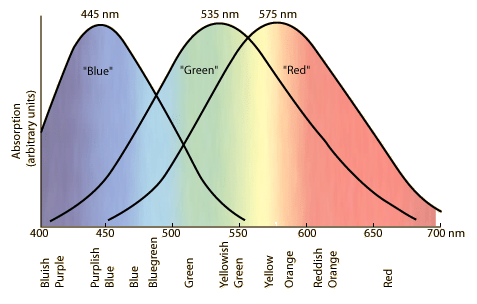
\includegraphics[scale=0.4]{images/RGB_cones.png}}
	\end{itemize}
	\item Colors are seen as variable combination of primary R, G and B colors	
\end{itemize}
\end{block}
\end{frame}
%--------------
\begin{frame}
\frametitle{Color fundamentals}
\begin{block}{Primary colors}
\begin{itemize}
	\item Specific wavelength to the three colors by CIE (International Commission on Illumination)designated: B (435.8 nm), G (546.1 nm) and R (700 nm)
	\item Secondary colors : adding the primary colors
	\begin{itemize}
	\item magenta (R+B), cyan (G+B), yellow (R+G)
	\end{itemize}
\end{itemize}
\begin{columns}
\column{0.5\textwidth}
Mixture of light\\	
	\centering{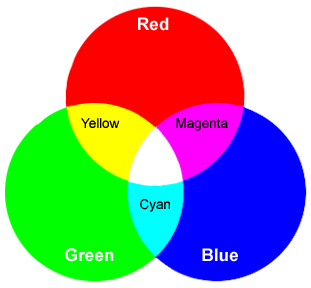
\includegraphics[width = 0.65\textwidth]{images/L6_primarycolors.png}}
\column{0.5\textwidth}
Mixture of pigments\\	
	\centering{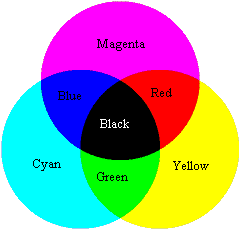
\includegraphics[width = 0.6\textwidth]{images/L6_secondarycolors.png} }
\end{columns}
\end{block}
\end{frame}
%------------
\begin{frame}
\frametitle{Color fundamentals}
\begin{block}{Color characteristics}
\footnotesize{
\begin{itemize}
\item \textit{Brightness} - embodies the achromatic notation of intensity
\item \textit{Hue} - associate with the dominant wavelength in a mixture of waves, represent the dominant color
\item \textit{Saturation} - relative purity or the amount of white light mixed with hue. 

\begin{itemize}
	\scriptsize{\item Pure spectrum colors are fully saturated 
	\item Degree of saturation and amount of added white light $\rightarrow$ inversely proportional
	}
\end{itemize}

\item \textit{Chromaticity} -  Hue and Saturation together
\item \textit{Tristimulus value} - amount of R,G and B to form any particular color ($X,Y,Z$)
\item \textit{Trichromatic color coefficients} - $x = \frac{X}{X+Y+Z}$, $y = \frac{Y}{X+Y+Z}$, $z= \frac{Z}{X+Y+Z}$, $x+y+z =1$
\end{itemize}
}
\end{block}
\end{frame}
%------------
\begin{frame}
\frametitle{Color fundamentals}
\begin{block}{CIE Chromaticity diagram}
\begin{itemize}
\item A method for specifying colors
\item Specific color composition as function of $x$(red) and $y$(green)
\item For any value of $x$ and $y$ $\rightarrow$ $z$ (blue) = $1 -x-y$
\end{itemize}
\end{block}
\end{frame}
%------------
\begin{frame}
\frametitle{Color fundamentals}
\begin{block}{CIE Chromaticity diagram}
\centering{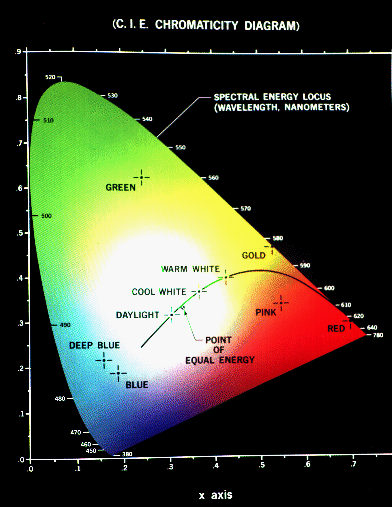
\includegraphics[width = 0.49\textwidth]{images/L6_CIEdiagram2.png}}
\end{block}
\end{frame}
%-----------------
%\begin{frame}
%\frametitle{Color fundamentals}
%\begin{block}{CIE Chromaticity diagram}
%\centering{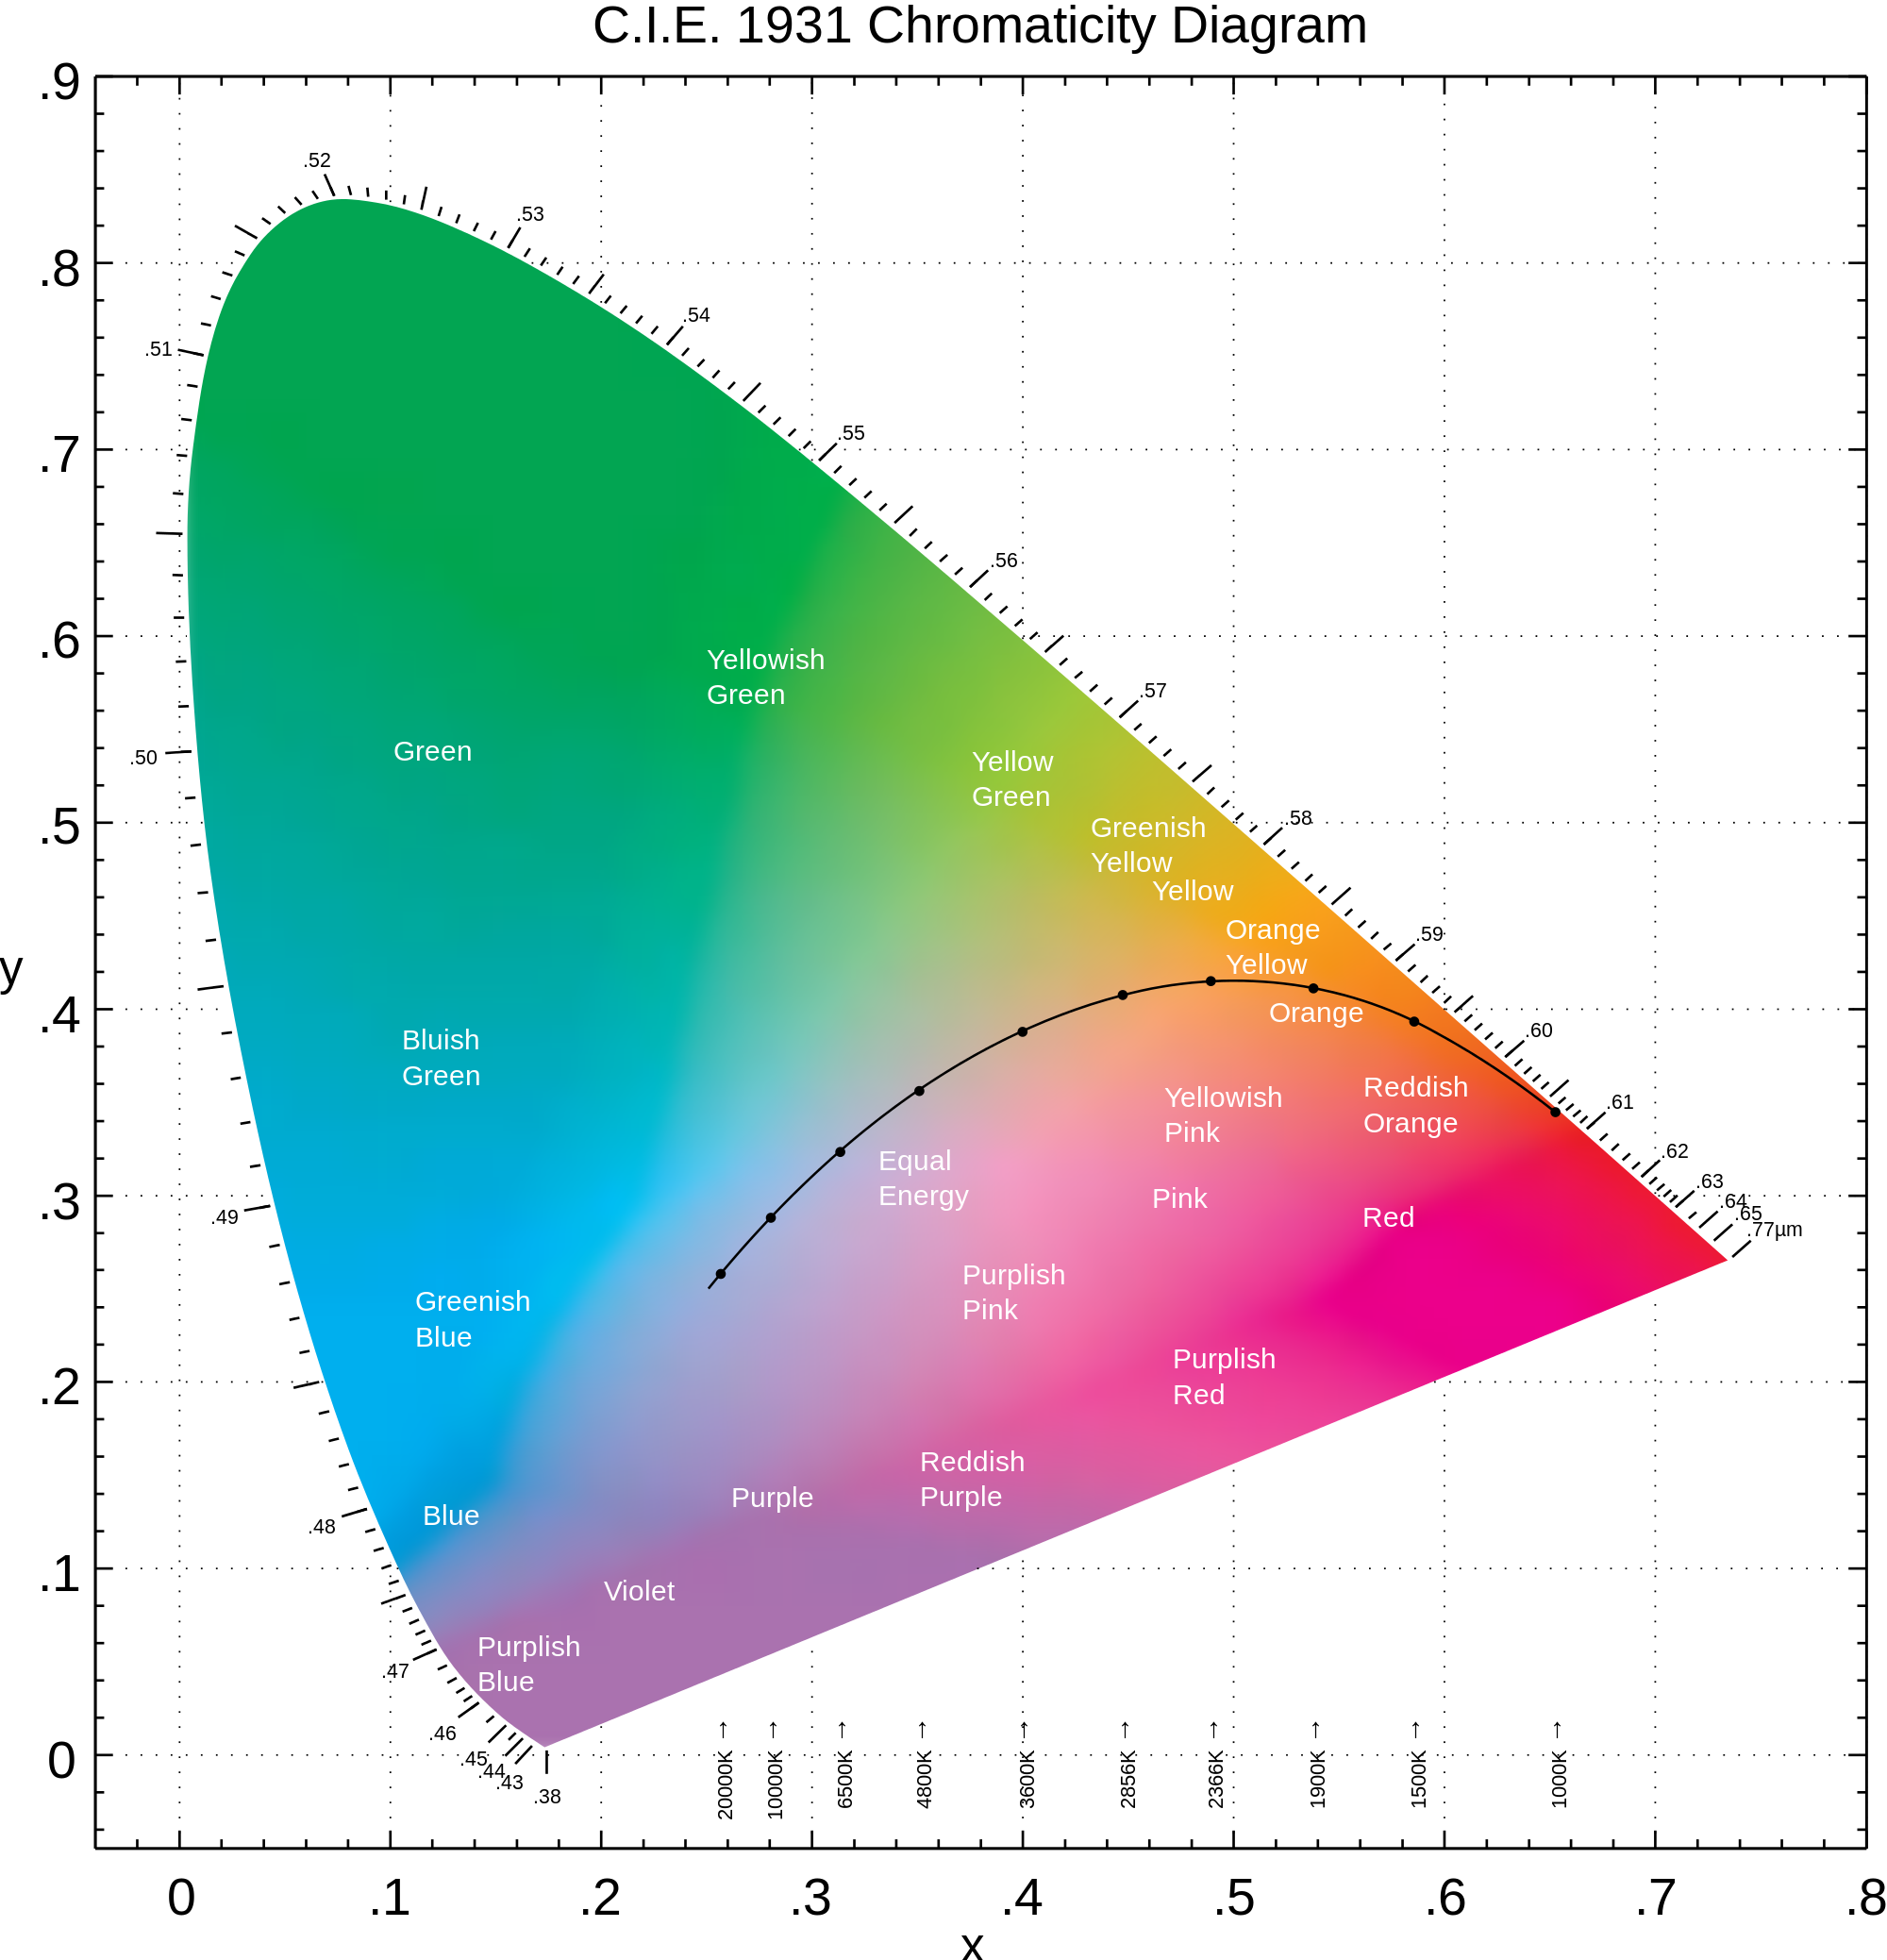
\includegraphics[width = 0.55\textwidth]{images/L6_CIEdiagram.png}}
%\end{block}
%\end{frame}
%---------------
\begin{frame}
\frametitle{Color fundamentals}
\begin{block}{CIE Chromaticity diagram}
\begin{itemize}
	\item Pure spectrum colors located around boundary 
	\item Non-boundary colors are mixture of spectrum colors
	\item The equal energy point represent the CIE standard for white light 
	\item A straight line joining any two point on the border, represent all the colors that can be created by mixing these two colors
\end{itemize}
\end{block}
\end{frame}
%-----------
\begin{frame}
\frametitle{Color fundamentals}
\begin{block}{CIE Chromaticity diagram}
\footnotesize{Typical color gamut of color monitors and color printers}
\centering{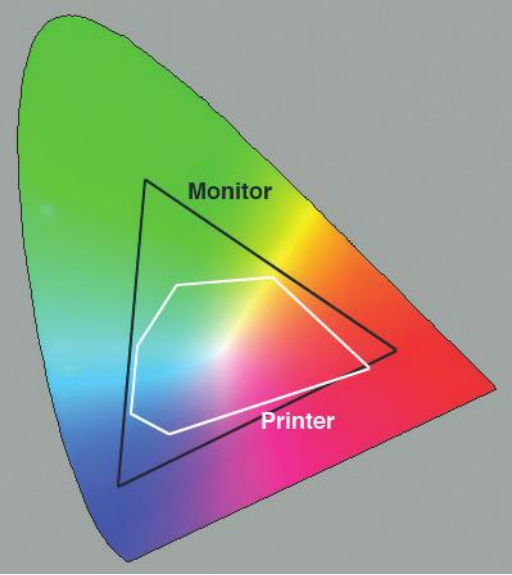
\includegraphics[scale=0.36]{images/L6_gamut_MP.png}}
\end{block}
\end{frame}
%-----------------
\section{Color models}
\begin{frame}
\frametitle{Color models}
\begin{itemize}
	\item Oriented towards hardware or application
	\item RGB (red, green, blue) model for color monitors and color video cameras
	\item CMY (cyan, magenta, yellow) and CMYK (cyan, magenta, yellow, black) for color printing
	\item HSI (hue, saturation, intensity), closer to human eyes, 
\end{itemize}
\end{frame}
%-------------
\begin{frame}
\frametitle{Color models}
\framesubtitle{RGB model}
\begin{block}{RGB model}
\footnotesize{
\begin{itemize}
\item Based on Cartesian coordinates 
\item Three axis, representing, red, green and blue
\item \textit{Bit depth} - number of bits representing each pixel in RGB 
\item 24 RGB bit depth - Total number of colors = $(2^8)^3$ = $16,777,216$
\end{itemize}
}
\begin{columns}
\column{0.5\textwidth}
\centering{
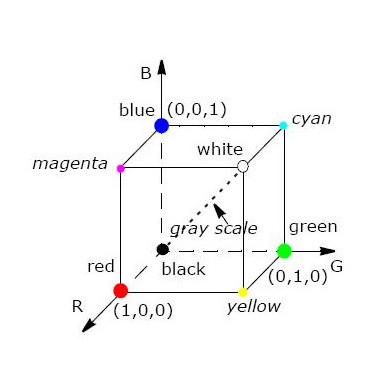
\includegraphics[width = 0.87\textwidth]{images/L6_RGB.jpg}
}
\column{0.5\textwidth}
\centering{
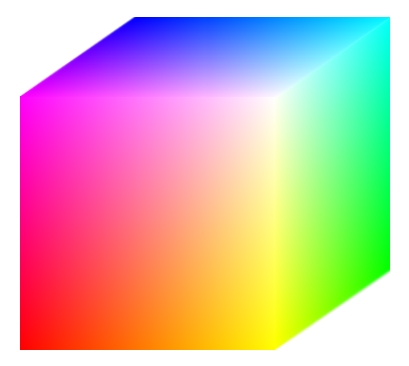
\includegraphics[width = 0.5\textwidth]{images/L6_RGBcube.jpg}
}
\end{columns}
\end{block}
\end{frame}
%-----------------
\begin{frame}
\frametitle{Color models}
\framesubtitle{RGB model}
\begin{block}{RGB model}
\footnotesize{XYZ $\rightarrow$ RGB}
\[
\begin{bmatrix}
R\\G\\B
\end{bmatrix} = 
\begin{bmatrix}
0.41847 & -0.15866 & - 0.082835\\
-0.091169 & 0.25243 & 0.015708 \\
0.00092090 & - 0.0025498 & 0.17860 
\end{bmatrix} 
.
\begin{bmatrix}
X\\Y\\Z
\end{bmatrix}
\]
\end{block}
\end{frame}
%----------------
\begin{frame}
\frametitle{Color models}
\framesubtitle{Lab model}
\begin{block}{Lab color space}
\begin{itemize}
\footnotesize{
\item Three components:
\item Luminance, brightness (L) and two chromatic components, one ranges from green to red, the other from blue to yellow
}
\end{itemize}
\begin{columns}
\column{0.3\textwidth}
\begin{center}
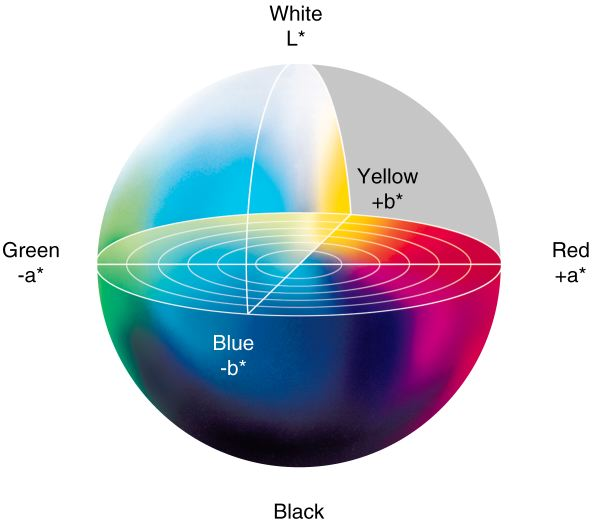
\includegraphics[scale=0.9]{images/L6_lab.jpg}
\end{center}
\column{0.55\textwidth}
\tiny{
$$ L^{\ast} = 116 f(Y/Y_{n})$$
$$a^{\ast} = 500[f(X/X_{n}) - f(Y/Y_{n})]$$
$$b^{\ast} = 200[f(Y/Y_{n}) - f(Z/Z_{n})]$$
where 
$$ f(t) = \begin{cases}
t^{1/3} & \text{   if  } t > (\frac{6}{29})^{3} \\
\frac{1}{3} (\frac{29}{3})^{2} t + \frac{4}{29} & \text{otherwise}
\end{cases}$$ 
$Y_{n}$, $X_{n}$ and $Z_{n}$, CIEXYZ tristimulus values of white reference point under illumination of D65

$$X_{n} = 0.95047, Y_{n} =1.0000 , Z_{n} = 1.08883 $$ 
}
\end{columns}
\end{block}
\end{frame}
%-----------------
\begin{frame}
\frametitle{Color models}
\framesubtitle{CMY model}
\begin{block}{CMY / CMYK model}
\footnotesize{
\begin{itemize}
\item Color printers and copies 
\item CMYK (four-color printing)
\item For normalized colors $\in [0, 1]$
\[
\begin{bmatrix}
C\\M\\Y
\end{bmatrix} =
\begin{bmatrix}
1\\1\\1
\end{bmatrix} -
\begin{bmatrix}
R\\G\\B
\end{bmatrix} \] 
\end{itemize}}
\vspace{-0.3cm}
\centering{
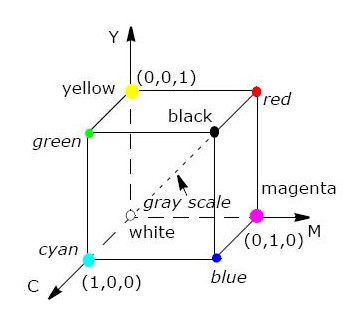
\includegraphics[width = 0.33\textwidth]{images/L6_CMY.jpg}
}
\end{block}
\end{frame}
%-----------------
\begin{frame}
\frametitle{Color models}
\framesubtitle{HSI model}
\begin{block}{HSI model}
\scriptsize{
\begin{itemize}
\item Closest to human color interpretation
\item \textbf{Hue} - Pure/dominant color
\item All colors on the plain defined by black/white line and one pure color have the same hue\\
\centering{
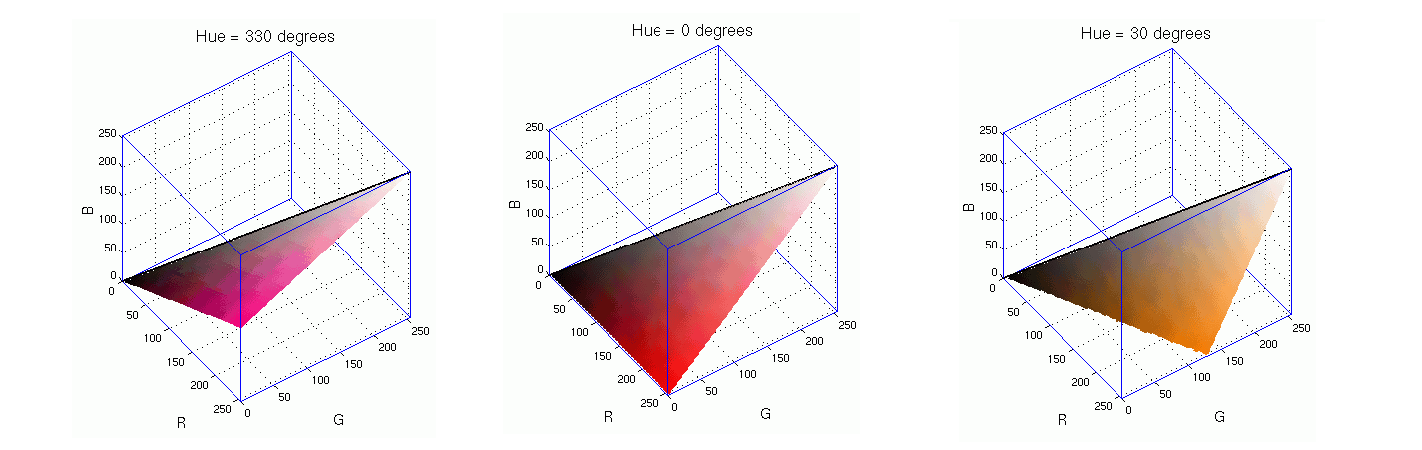
\includegraphics[width = 0.9\textwidth, height = 0.3\textheight]{images/L6_Hue_RGB_1.png}}
\end{itemize}}
\end{block}
\end{frame}
%---------------
\begin{frame}
\frametitle{Color models}
\framesubtitle{HSI model}
\begin{block}{HSI model}
\scriptsize{
\begin{itemize}
\item \textbf{Saturation} - Purity, amount of white light mixed with hue
\item Distance form associated pure color (perpendicular distance to the black/white line)
\item points further away from this line are more saturated, then the one closer\\
\centering{
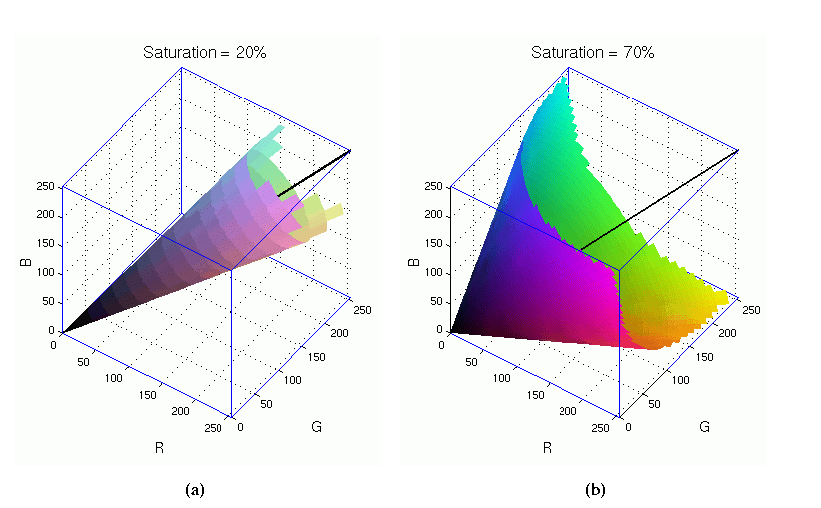
\includegraphics[scale = 0.27]{images/L6_S_RGB_1.png}}
\end{itemize}}
\end{block}
\end{frame}
%---------------
\begin{frame}
\frametitle{Color models}
\framesubtitle{HSI model}
\begin{block}{HSI model}
\scriptsize{
\begin{itemize}
\item \textbf{Intensity} - Brightness
\item How much light an object is emitting
\item Colors on the plane perpendicular on black/white line, where $R+G+G =k$ have the same brightness\\
\centering{
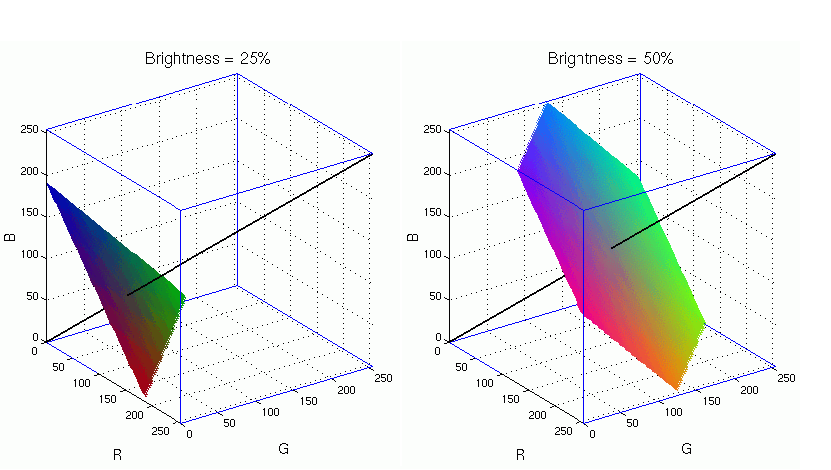
\includegraphics[scale = 0.27]{images/L6_I_RGB_1.png}}
\end{itemize}}
\end{block}
\end{frame}
%--------------
\begin{frame}
\frametitle{Color models}
\framesubtitle{HSI model}
\begin{block}{HSI model}
\scriptsize{
\begin{itemize}
\item Relations between RGB cube and HSI 
\item[]
\centering{
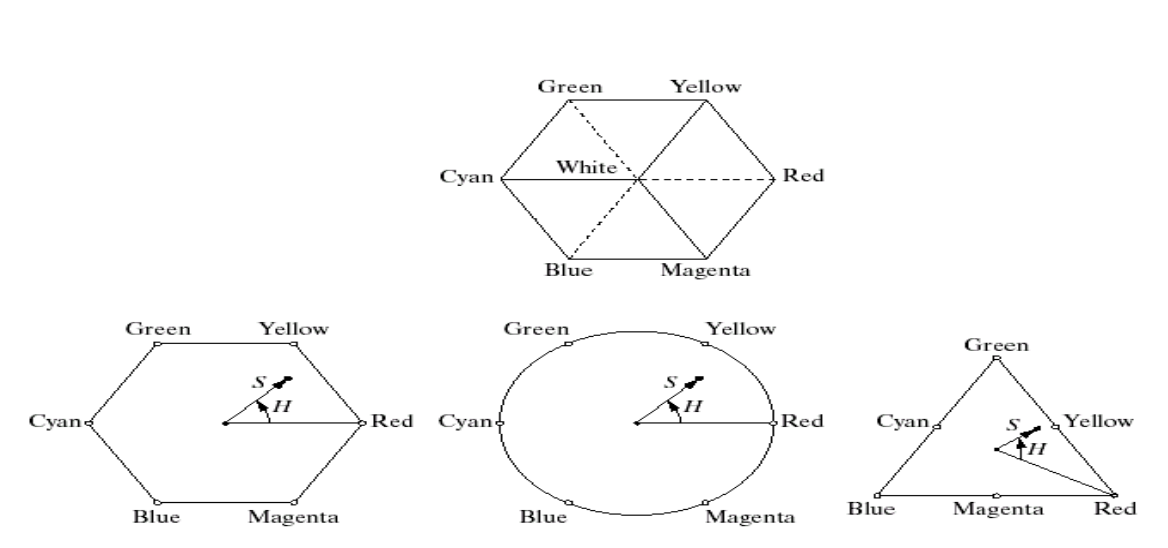
\includegraphics[width = 0.8\textwidth]{images/L6_HSI_RGB2.png}}
\end{itemize}}
\end{block}
\end{frame}
%---------------
\begin{frame}
\frametitle{Color models}
\framesubtitle{HSI model}
\begin{block}{HSI model}
\scriptsize{
\begin{itemize}
\item Relations between RGB cube and HSI 
\item[]
\centering{
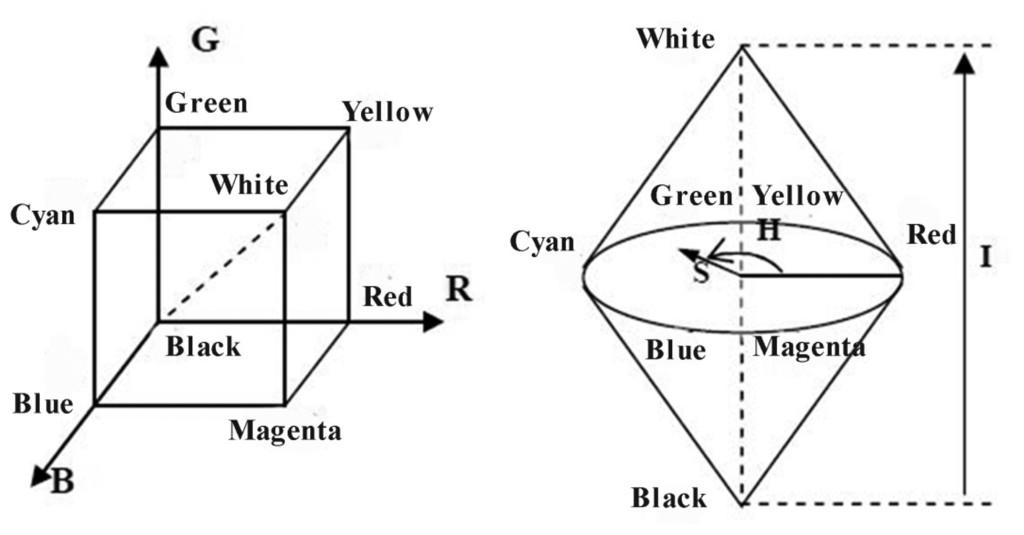
\includegraphics[width = 0.9\textwidth]{images/L6_HSI_RGB.png}}
\end{itemize}}
\end{block}
\end{frame}
%---------------
\begin{frame}
\frametitle{Color models}
\framesubtitle{HSI model}
\begin{block}{RGB $\rightarrow$ HSI}
\centering{
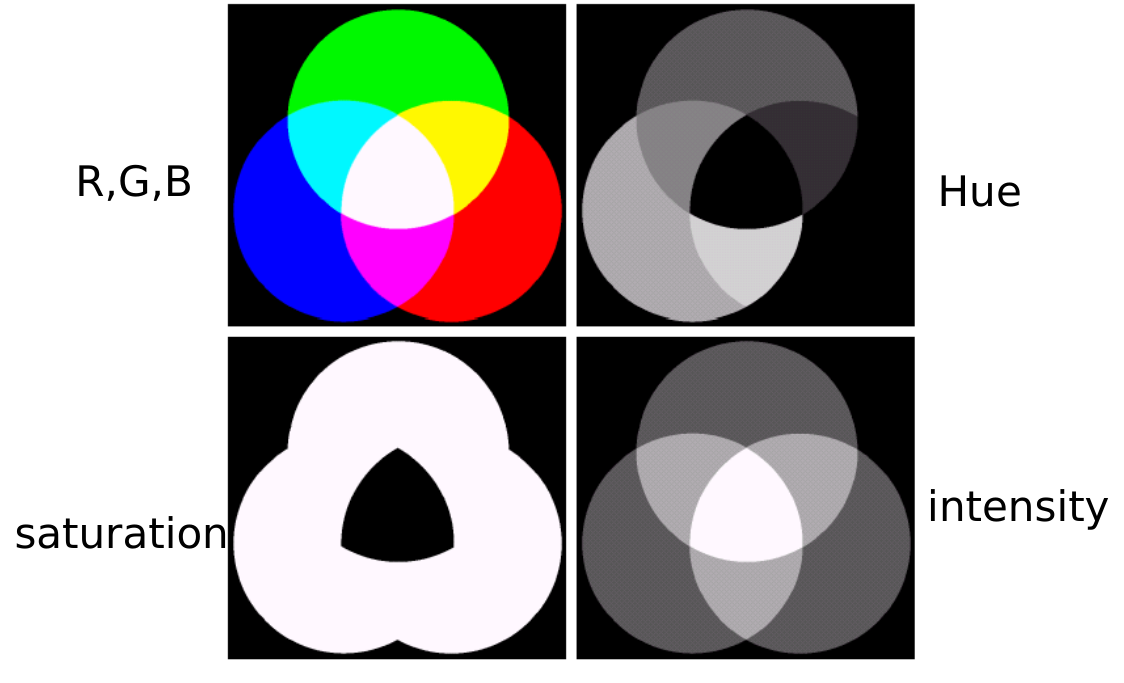
\includegraphics[width = 0.9\textwidth]{images/L6_HSI_RGB3.png}}
\end{block}
\end{frame}
%---------------
\begin{frame}
\frametitle{Color models}
\framesubtitle{HSI model}
\begin{block}{Conversion from RGB to HSI}
\scriptsize{
\begin{itemize}
\item[] 
\[ H = 
\begin{cases} 
   	0 & \text{if } B \geq G \\
   	360-\theta & \text{if } B > G
  	\end{cases}
\]
\[
\theta = \cos^{-1}\lbrace\frac{\frac{1}{2}(R-G)+(R-B)}{[(R-G)^{2}+(R-B)(G-B)]^{1/2}}\rbrace
\]
\item[]
\[
S = 1 -\frac{3}{(R+G+B)}[\min(R,G,B)] 
\]
\item[]
\[
I = \frac{R+G+B}{3}
\]
\end{itemize}}
\end{block}
\end{frame}
%-------------
\begin{frame}
\frametitle{Color models}
\framesubtitle{HSI model}
\begin{block}{Conversion from HSI to RGB}
\scriptsize{
\begin{itemize}
\item re-arrange H $\in [0, 360^{\circ}]$ 
\item[]
\[\text{RG sector  , } 
0^{\circ} \leq H < 120^{\circ} \rightarrow
\begin{cases}
B = I(1-S)\\
R =  I[1+\frac{S\cos H}{\cos(60^{\circ}-H)}]\\
G = 3I - (R+B)
\end{cases}
\]
\item[]
\[ \text{GB sector  , } 
120^{\circ} \leq H < 240^{\circ} \rightarrow
\begin{cases}
H = H - 120^{\circ}\\
R = I(1-S)\\
G =  I[1+\frac{S\cos H}{\cos(60^{\circ}-H)}]\\
B = 3I - (R+G)
\end{cases}
\]
\item[]
\[ \text{BR sector  , } 
240^{\circ} \leq H < 360^{\circ} \rightarrow
\begin{cases}
H = H - 240^{\circ}\\
G = I(1-S)\\
B =  I[1+\frac{S\cos H}{\cos(60^{\circ}-H)}]\\
R = 3I - (G+B)
\end{cases}
\]
\end{itemize}}
\end{block}
\end{frame}
%--------------
\begin{frame}
\frametitle{Color models}
\framesubtitle{Example of RGB, HSI and CMYK}
\begin{center}
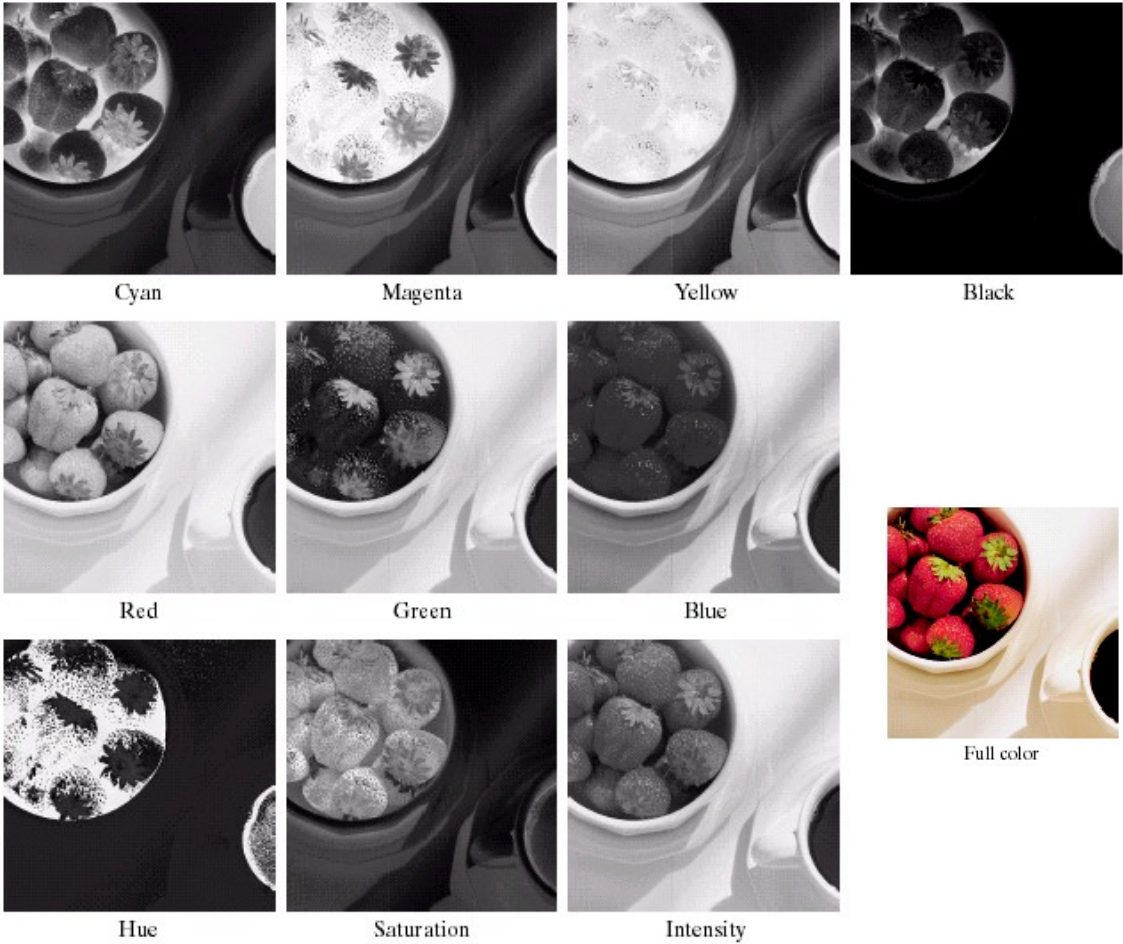
\includegraphics[scale= 0.27]{images/L6_ex_RGBCYMHSI.png}
\end{center}
\end{frame}
%--------------
\begin{frame}
\frametitle{Color models}
\framesubtitle{HSL and HSV}
\begin{itemize}
\item \textit{HSL} stands for hue, saturation and lightness
\item \textit{HSV} stands for hue, saturation and value
\end{itemize}
\begin{center}
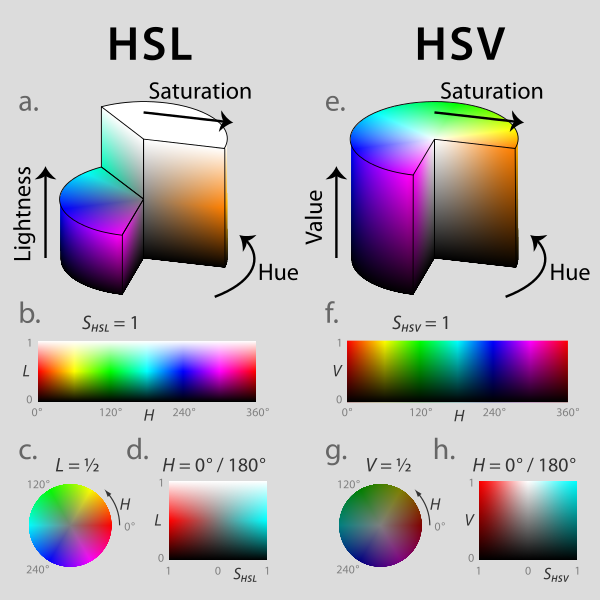
\includegraphics[scale=0.26]{images/L6_HSLHSV1.png}
\end{center}
\end{frame}

%--------------
\begin{frame}
\frametitle{Color models}
\framesubtitle{HSL and HSV}
\footnotesize{
 In both colorspace: 
\begin{itemize}
	\item Hue is the angle around the central vertical axis
	\item Saturation is the distance from the axis
	\item Lightness or value are the distance along the axis
	\item Hue is the same, while \textbf{saturation} differs dramatically
	\item[]
	\begin{center}	
	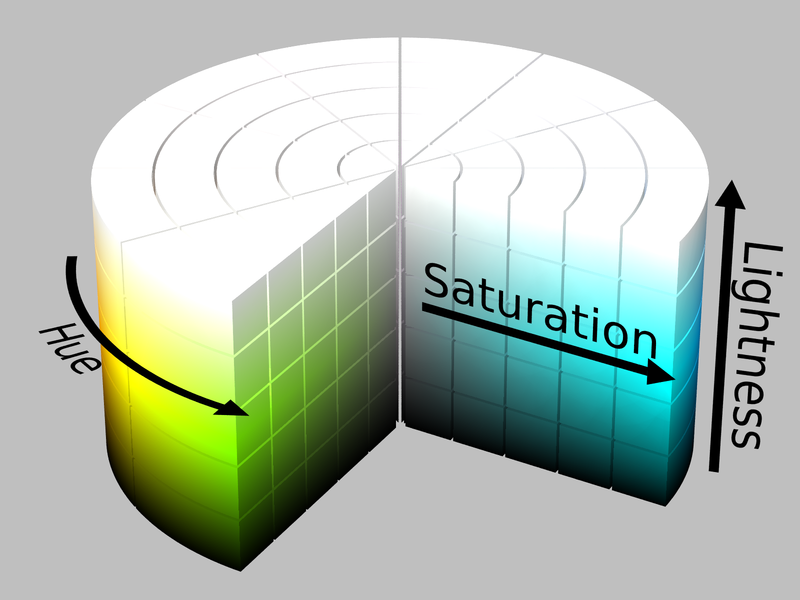
\includegraphics[scale=0.06]{images/L6_HSL1.png}\
	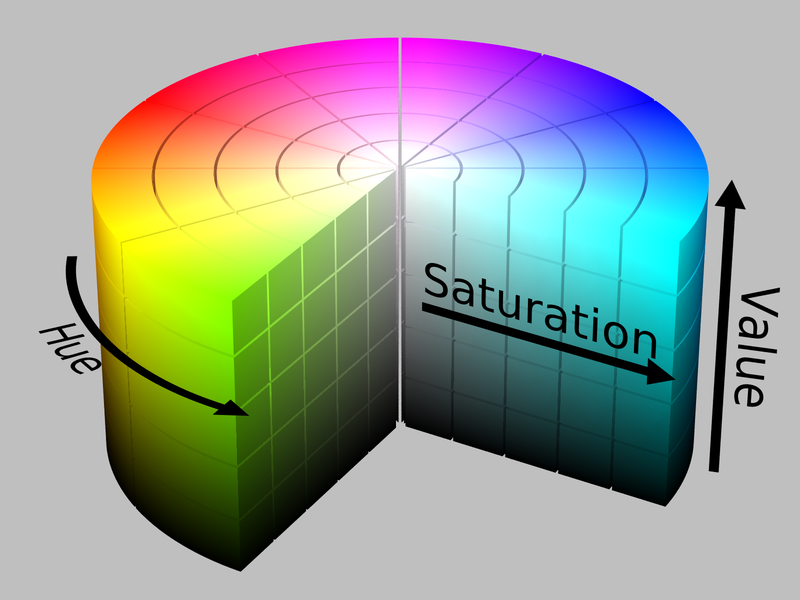
\includegraphics[scale=0.06]{images/L6_HSV1.png}
	\end{center}
	
	\item Plotting the hue and lightness and value against chroma rather than saturation
	\item[]
	\begin{center}
	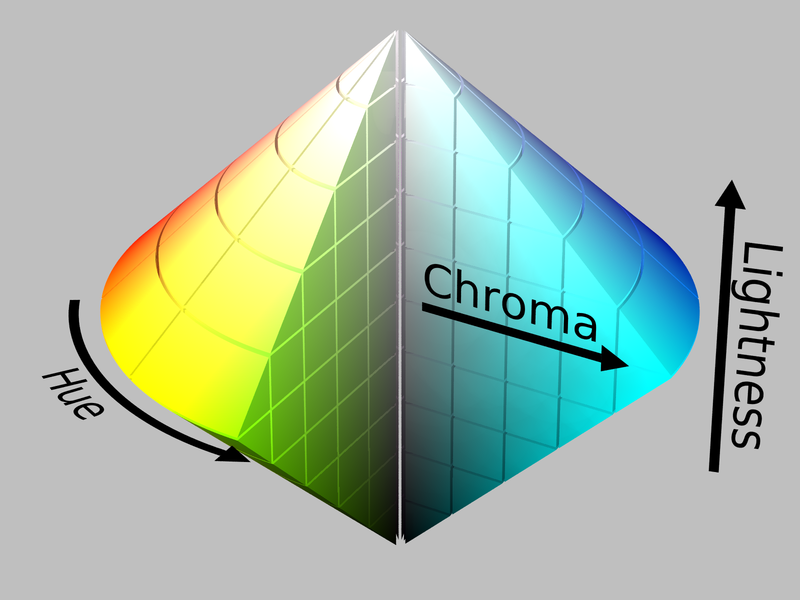
\includegraphics[scale=0.06]{images/L6_HSL2.png}\
	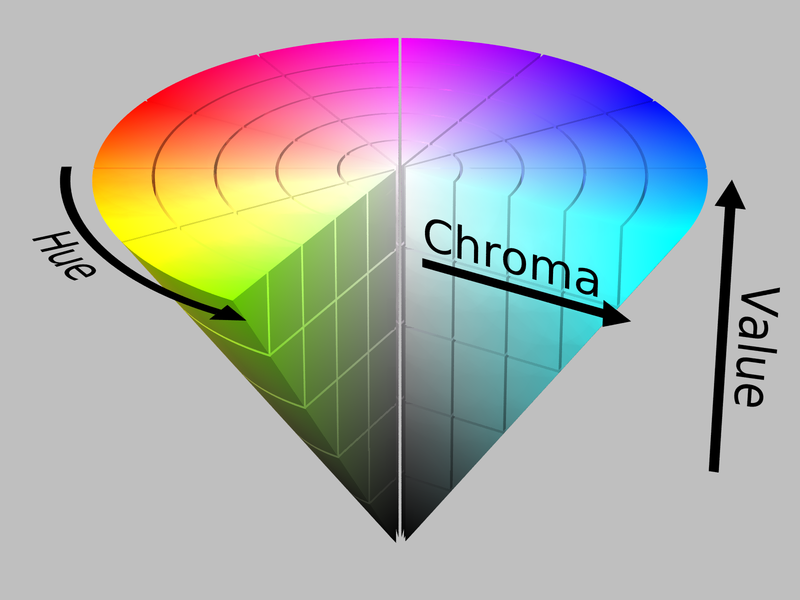
\includegraphics[scale=0.06]{images/L6_HSV2.png}
	\end{center}	
\end{itemize}
}
\end{frame}
%--------------
\begin{frame}
\frametitle{Color models}
\framesubtitle{HSL and HSV}
\begin{itemize}
\footnotesize{
	\item Chroma: The ``colorfulness relative to the brightness of a similarly illuminated white''
	\item $C = \frac{OP}{OP'}$ 
	\item[]
	\begin{center}
	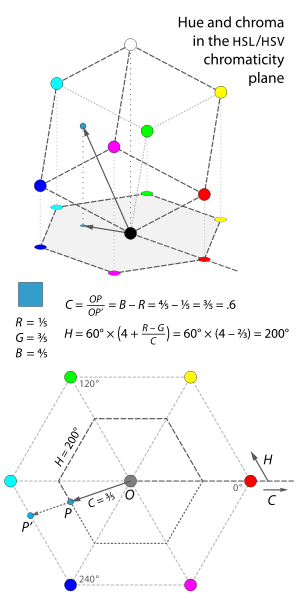
\includegraphics[height = 0.6\textheight]{images/L6_ChromaH.png}
	\end{center}
		}
\end{itemize}
\end{frame}
%--------------
\begin{frame}
\frametitle{Color models}
\framesubtitle{HSI vs. HSL vs. HSV}
\footnotesize{
$$ I = \frac{R+G+B}{3}$$
$$ V = \max(R,G,B)$$
$$ L = \frac{\min(R,G,B) + \max(R,G,B)}{2} $$
$$ S_{HSI} = 
\begin{cases}
0 & \text{ if  } C = 0\\
1- \frac{m}{I} & \text{otherwise}
\end{cases} $$ 
$$ S_{HSV} = 
\begin{cases}
0 & \text{ if  } C = 0\\
\frac{C}{V} & \text{otherwise}
\end{cases}$$   
$$ S_{HSL} = 
\begin{cases}
0 & \text{  if  } C = 0\\
\frac{C}{1-\vert 2L - 1\vert} & \text{otherwise}
\end{cases} $$
}
\end{frame}
%--------------
\section{Pseudocolor image processing}
\begin{frame}
\frametitle{Pseudocolor image processing}
\begin{itemize}
\item Pseudocolor (false color) is assigning color to gray values based on a specified criteria 
\item $\rightarrow$ Converting gray images to color
\item \textbf{Why ?} improve the visualization and since human can discern thousands of color shades but only two dozen gray shades  
\end{itemize}
\begin{block}{Techniques}
\begin{itemize}
\item Intensity slicing
\item Intensity to color transformation
\end{itemize}
\end{block}
\end{frame}
%---------------
\begin{frame}
\frametitle{Pseudocolor image processing}
\begin{block}{Intensity slicing}
\footnotesize{
\begin{itemize}
\item Assume $[0, L-1]$ represent the gray scale of gray image $I$
\item Let $l_{0}$ represent black level $[f(x,y) = 0 ]$ and $l_{L-1}$ represent white level $[f(x,y) = L-1]$
\item Suppose that $P$ planes perpendicular to the intensity axis are defined at levels $l_{1}, l_{2}, ..., l_{p}$
\item Assuming that $0 < P < L-1$, the $P$ planes partition the gray scale into $P+1$ intervals $V_{1}, V_{2}, ..., V_{P+1}$
\item Intensity to color are made based on : 
$$ f(x,y) = c_{k} \text{,  if } f(x,y)\in V_{k} $$
\item $c_{k}$ is the color associated with the $k^{th}$ intensity interval $V_{k}$
\end{itemize}
}
\end{block}
\end{frame}
%-------------
\begin{frame}

\frametitle{Pseudocolor image processing}
\begin{block}{Intensity slicing}
\footnotesize{
\begin{itemize}
\item Assuming 3D representation of image, considering the intensity as $z$ axis 
\end{itemize}
}
\centering{
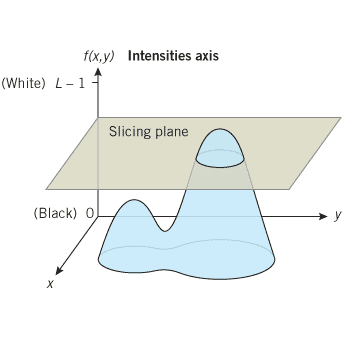
\includegraphics[height = 0.65\textheight]{images/L6_intensityslicing.png}}
\end{block}
\end{frame}
%-------------
\begin{frame}
\frametitle{Pseudocolor image processing}
\begin{block}{Intensity slicing}
\begin{itemize}
\footnotesize{\item Monochrome Xray image and result of color coding}
\centering{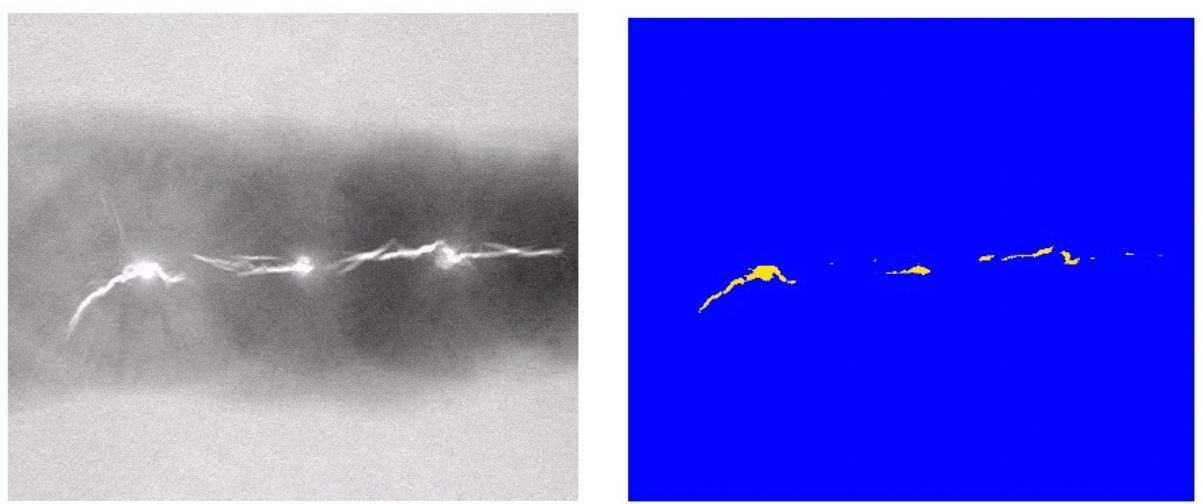
\includegraphics[scale= 0.3]{images/L6_ex_intensityslicing.png}}
\end{itemize}
\end{block}
\end{frame}
%-------------
\begin{frame}
\frametitle{Pseudocolor image processing}
\begin{block}{Intensity to color transformation}
\begin{itemize}
\item Intensity slicing, limits range of pseudocolor enhancement result
\item To have a wider range of pseudocolor enhancement $\rightarrow$ process gray image using independent transformation ($R,G,B$) and combine the results to create one color image
\end{itemize}
\centering{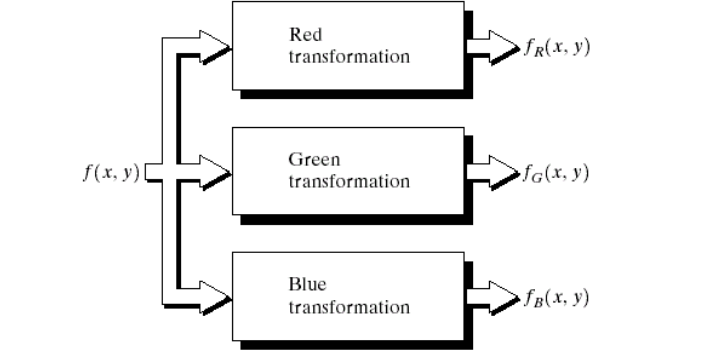
\includegraphics[scale=0.35]{images/L6_ICT.png}}
\end{block}
\end{frame}
%------------
\begin{frame}
\frametitle{Pseudocolor image processing}
\begin{block}{Intensity to color transformation}
\begin{columns}
\column{0.5\textwidth}
\centering{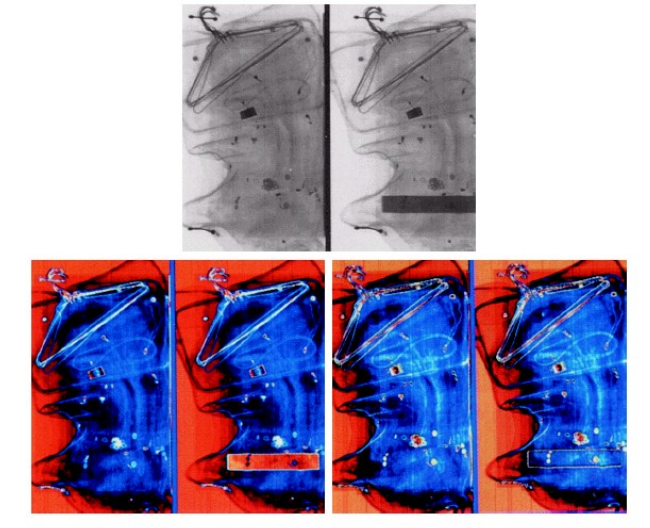
\includegraphics[scale=0.3]{images/L6_ex_ICT1.png}}
\column{0.5\textwidth}
\centering{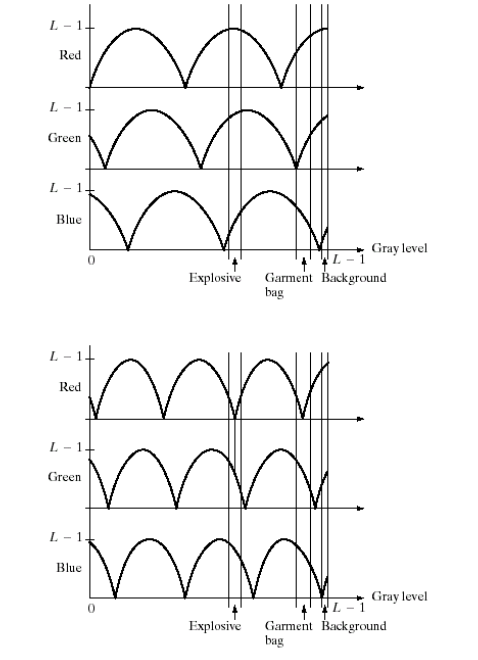
\includegraphics[scale=0.35]{images/L6_ex_ICT2.png}}
\end{columns}
\end{block}
\end{frame}
%------------
\section{Color Transformation}
\begin{frame}
\frametitle{Color transformation}
\footnotesize{
\begin{itemize}
\item[]
$$g(x,y) = T[f(x,y)] $$
\item $f(x,y)$ is the color input, $g(x,y)$ is the transformed color output, and $T$ is an operator on $f$ over a spatial neighborhood of $(x,y)$ 
\item In theory, any transformation can be applied in any color model, however in practice some operation are suited to some models than others
\item E.g. Modifying the intensity of the image using $g(x,y) = kf(x,y)$, for $ 0 < k < 1$
\scriptsize{
\begin{itemize}
	\item \textit{HSI} - $s_{3} = kr_{3}$, and $s_{2} = r_{2}$ , $s_{1} = r_{1}$
	\item Only HSI intensity $r_{3}$ is modified 
	\item \textit{RGB} - $s_{i} = kr_{i}$, $i = 1,2,3$
	\item \textit{CMY} - $s_{i} = kr_{i}+(1-k)$, $i = 1,2,3$
\end{itemize}
}
\end{itemize}
}
\end{frame}
%------------
\begin{frame}
\frametitle{Color transformation}
\footnotesize{Adjusting the intensity of color image and the required RGB, HSI and CMY transfer function}\\
\centering{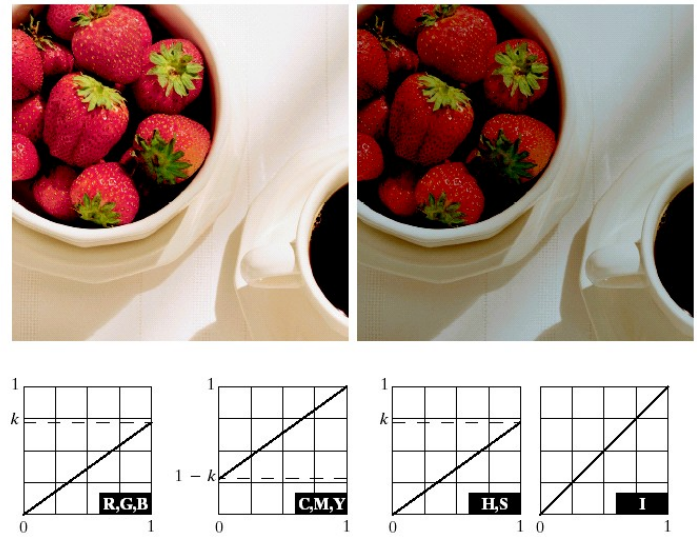
\includegraphics[scale=0.35]{images/L6_ex_CT.png}}\\
{\color{red} The H,S and I caption should be switch }
\end{frame}
%------------
\begin{frame}
\frametitle{Colro transformation}
\framesubtitle{Histogram equalization}
\footnotesize{
\begin{itemize}
\item Adapting the mono-channel histogram equalization to color-channels are not wise and cause erroneous colors
\item More suitable approach : spreading the color intensities uniformly and leaving the color themselves (e.g, hue) unchanged 
\end{itemize}
}
\begin{center}
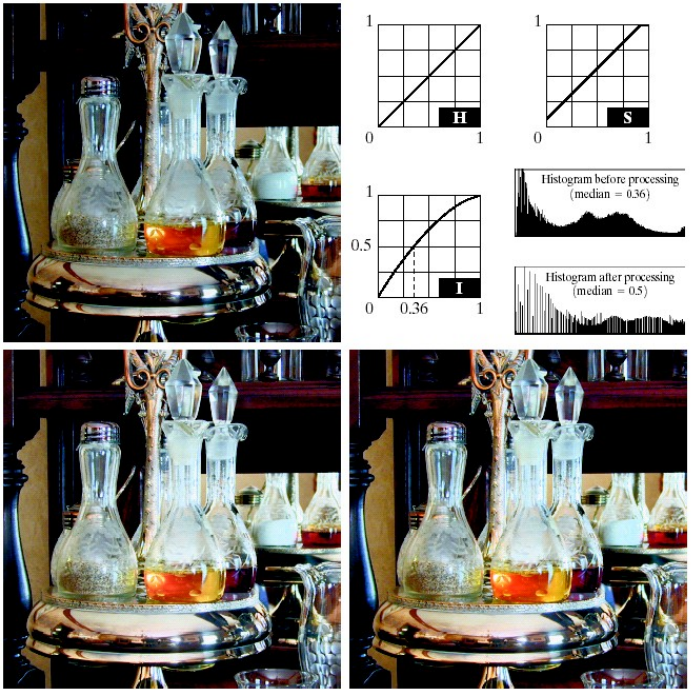
\includegraphics[scale=0.23]{images/L6_ex_HE_color.png}
\end{center}
\end{frame}
%-------------
\section{Demosaicing}

%--------------


\end{document}

%\begin{itemize}
%\item Also use neighborhood but do not use coefficients 
%\begin{itemize}
%\item median filter for noise reduction
%\end{itemize} 
%\end{itemize}
